\subsection{ISAC Pipeline System Architecture}
\label{subsec:isac_pipeline}

The proposed Integrated Sensing and Communication (ISAC) pipeline system architecture, presented in Figure \ref{fig:isac-pipeline-architecture}, is designed to seamlessly integrate environmental sensing and adaptive beamforming for enabling dynamic, direction-aware communication into a cohesive framework.
There are four main modules in the ISAC pipeline: the Sensing Module, the Multi-Target Tracking Module, the Adaptive Beamforming Module, and the Communication Module.

The \textbf{Sensing Module} is responsible for capturing and processing the radio propagation signals from the environment, to detect the objects in the environment and estimate their states, including position, and velocity.
In order to achieve this, the sensing module use the MIMO antennas as the monostatic radar antennas to transmit and receive the radio signals.
It begins by emitting rays from the transmitter (Tx) and the receiver (Rx) captures the reflected rays from the environment.
From the received reflected rays, it extract essential information such as delay, power, Direction of Arrival (DoA), etc and it calculate the 3D Equivalent Reflection Point (ERP), estimating the exact physical origin of the bounce rays.
To eliminate the unwanted reflections from the structural noises from the environment such as floor and ceiling, a spatial filter is applied to filter out rays that orginated outside the a defined vertical region of interest and this process is called Z-filtering.
After rays from the floor and ceiling are filtered out,the Moving Target Indicator (MTI) Filter is applied to filter out the rays reflected from the static objects in the environment such as pillars and walls.
Finally, the Density-Based Spatial Clustering of Applications with Noise (DBSCAN) algorithm is applied on the remaining rays in order to identify and group the rays into clusters that correspond to distinct objects in the environment.
The centroid of each cluster is calculated and used as the estimated position of the object (i.e., raw detection).

\begin{figure}[t]
  \centering
  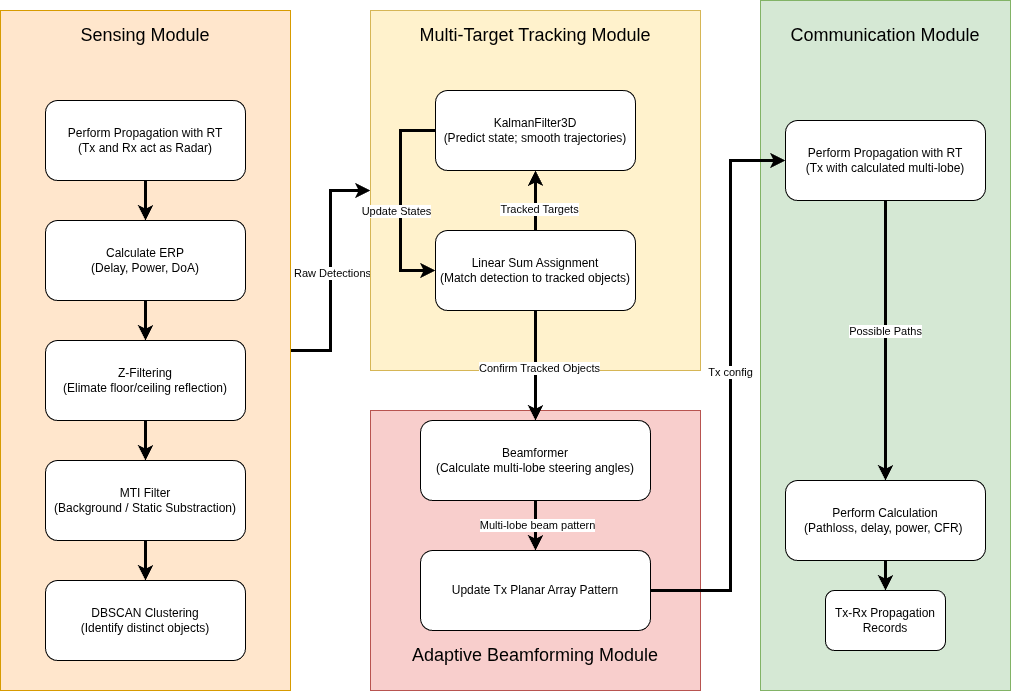
\includegraphics[width=\columnwidth]{images/isac_pipeline_architecture.png}
  \caption{ISAC Pipeline System Architecture.}
  \label{fig:isac-pipeline-architecture}
\end{figure}

These raw detections are then passed to the \textbf{Multi-Target Tracking Module}, which is responsible for monitoring the dynamic states of moving objects over time.
It utilizes a Linear Sum Assignment algorithm to optimally match incoming raw detections with previously tracked objects that are kept in the memory.
Matched detections are then passed to a 3D Kalman Filter, which predict the future state (e.g. position) of objects and make the transition of movement along their trajectories smooth.
This recursive loop continuously updates the tracked states of the objects, resulting in a refined set of confirmed tracked objects.

When the moving objects in the environment are detected and tracked successfully, the information of the detected objects can be used to form beams towards the detected objects to improve the quality of the communication link.
Based on the estimated position, velocity, and direction of the detected objects, the Beamformer of the \textbf{Adaptive Beamforming Module} calculate the multi-lobe steering angles required to directed beams towards the identified objects.
The multi-lobe beam pattern calculated is then used to update the Tx array configuration to focus the beams towards the detected objects.

Finally, the \textbf{Communication Module} calculate propagation in the channel  with the calculated multi-lobe beam pattern.
The module calculate propagation metrics such as pathloss, delay, received power, and Channel Frequency Response (CFR) based on the multi-lobe beam pattern.
These extracted propagation related information are then forwarded to ns-3 simulator to perform the communication simulation.